\documentclass[12pt]{article}

\usepackage{tikz}
\usepackage{geometry}

\usetikzlibrary{mindmap}

\pagestyle{empty}

\geometry{landscape, margin=1cm}


\begin{document}
\begin{center}
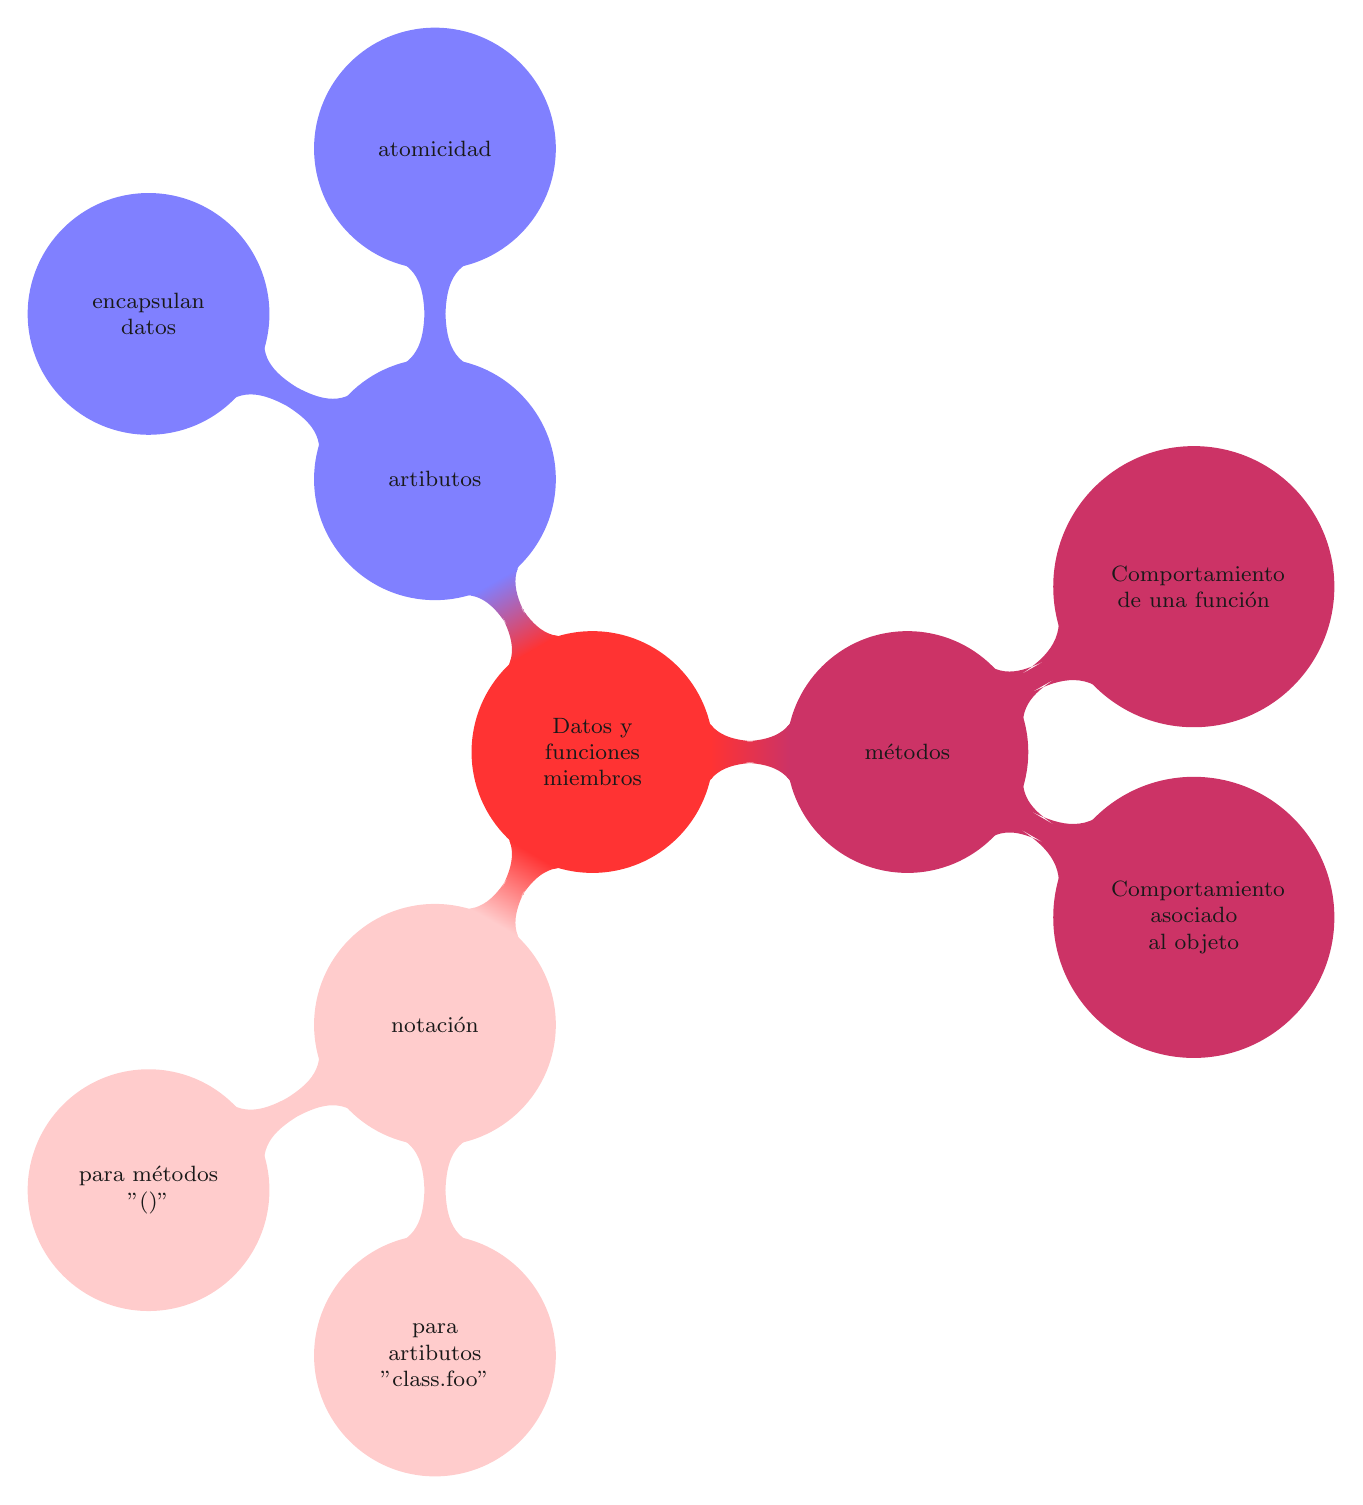
\begin{tikzpicture}[small mindmap, grow cyclic, every node/.style=concept, concept color=red!80, text=black!90, minimum size=3.0cm,
    level 1/.style={level distance=4.5cm,sibling angle=360/4},
    level 1/.style={level distance=4.0cm,sibling angle=360/3},
    level 2/.style={level distance=4.2cm,sibling angle=60},
    level 3/.style={level distance=3.5cm,sibling angle=60},
    ]

    \node{Datos y funciones\\miembros}
    child[concept color=pink!80] { node {notación}
        child { node {para métodos "()"} }
        child { node {para\\artibutos "class.foo"} }
    }
    child[concept color=purple!80] { node {métodos}
        child[minimum size=3.5cm] { node {Comportamiento asociado al objeto} }
        child[minimum size=3.5cm] { node {Comportamiento de una función} }
    }
    child[concept color=blue!50] { node {artibutos}
        child { node {atomicidad} }
        child { node {encapsulan datos} }
    }
    ;
\end{tikzpicture}
\end{center}
\end{document}
